\documentclass[11pt,a4paper]{article}

\usepackage[utf8]{inputenc}
\usepackage[T1]{fontenc}
\usepackage{amsmath}
\usepackage{amssymb}
\usepackage{geometry}
\usepackage{graphicx}
\usepackage{hyperref}
\usepackage{natbib}
\usepackage{booktabs}
\usepackage{multirow}
\usepackage{xcolor}
\usepackage{enumitem}
\usepackage{caption}
\usepackage{algorithm}
\usepackage{algorithmic}

\geometry{margin=1in}

\hypersetup{
    colorlinks=true,
    linkcolor=blue!60!black,
    citecolor=blue!60!black,
    urlcolor=blue!60!black
}

\title{\textbf{Role Adherence: A Metric for Evaluating Role Consistency\\
in Multi-Turn Conversational AI}}

\author{
    Axel Fritz\\
    \texttt{axel.fritz@alquimia.ai}\\
    Alquimia AI
    \and
    Alex Fiorenza\\
    \texttt{alex.fiorenza@alquimia.ai}\\
    Alquimia AI
}

\date{April 2026}

\begin{document}

\maketitle

\begin{abstract}
As conversational AI systems are deployed in role-constrained settings ---
customer support agents, educational tutors, medical assistants --- measuring
whether a model consistently adheres to its assigned role becomes a core quality
requirement. This paper proposes \textbf{Role Adherence}, a metric for the
Gaussia evaluation framework that quantifies role consistency across multi-turn
conversations under a constructive definition: an assistant must actively exhibit
the behaviour its role demands, not merely avoid out-of-scope content.

We evaluate eight scoring methods on a controlled synthetic benchmark of
150 turns (scope violations, tone violations, and constructive failures)
across three dataset-size conditions ($n \in \{15, 50, 150\}$). Key findings:
(1)~An LLM judge (\texttt{llama-3.3-70b-versatile}) achieves $F_1 = 0.979$
at $n \geq 50$ with tight bootstrap confidence intervals [$0.952$,\,$1.000$],
and is the only method that reads the role definition directly.
(2)~Cosine similarity and $k$-NN reach AUC\,$\approx 1.0$ on the benchmark,
but this is a structural artefact: deterministic metrics measure semantic
proximity to a ground-truth reference, not role adherence per se --- a tone
violation can be semantically indistinguishable from a role-adherent response.
(3)~Mahalanobis Distance in 384-dimensional embedding space \emph{degrades}
as $n$ grows (AUC: $0.963 \to 0.856$), confirming the curse of dimensionality.
(4)~A PCA-based dimensionality reduction intended to address this problem
inverts the adherence signal entirely (AUC\,$= 0.000$ at $n = 15$).
(5)~KL Divergence provides near-random signal at small $n$ (AUC\,$= 0.537$)
and converges weakly at large $n$ (AUC\,$= 0.877$), operating at the wrong
level of abstraction. The metric uses an LLM-as-a-judge as its default scoring path, as it is
the only method capable of reading the role definition and detecting tone
violations and constructive failures. Deterministic semantic methods are
available as a reproducible, cost-free alternative when ground truth is
present, but empirical results show they act as \emph{semantic drift
detectors} rather than genuine role adherence evaluators --- a distinction
with direct consequences for production deployments.
\end{abstract}

% ---------------------------------------------------------------------------
\section{Introduction}
% ---------------------------------------------------------------------------

Modern LLM-based assistants are typically deployed with a system prompt that
defines their role: the topics they should cover, the tone they should adopt,
the behaviours they should exhibit, and the boundaries they should respect.
Despite this, models frequently deviate from their assigned roles --- answering
out-of-scope questions, abandoning their defined persona, or failing to exhibit
the behaviour their role requires.

Existing evaluation frameworks either measure role adherence at the level of
individual turns in isolation \citep{zheng2023judging}, or rely entirely on
LLM-based judges, which introduce reproducibility and cost concerns
\citep{deriu2021survey}. This paper proposes a more complete metric that evaluates adherence across
the full conversational context, uses an LLM-as-a-judge as its default
scoring path, and offers deterministic semantic scoring as a reproducible
alternative when ground-truth reference responses are available.

% ---------------------------------------------------------------------------
\section{Problem Statement}
% ---------------------------------------------------------------------------

Given a multi-turn conversation between a user and an AI assistant, and a
definition of the role the assistant is expected to play, we want to compute a
scalar score representing how consistently the assistant adhered to that role
throughout the conversation.

Let a conversational session be a sequence of assistant turns
$t_1, t_2, \ldots, t_n$, and let $R$ denote the role definition. The Role
Adherence score is defined as:

\begin{equation}
  \text{RoleAdherence}(R, T) = \frac{1}{n} \sum_{i=1}^{n}
  \text{adhere}(t_i,\; T_{<i},\; R)
  \label{eq:score}
\end{equation}

where $T_{<i}$ is the conversation history up to turn $i$, and
$\text{adhere}(\cdot) \in [0, 1]$ is a per-turn adherence score. The
session score lies in $[0, 1]$, where 1 indicates full adherence across
all turns. The range of $\text{adhere}(\cdot)$ and how it is computed
depend on the scoring path selected (Section~\ref{sec:scoring}).

% ---------------------------------------------------------------------------
\section{Defining Adherence}
\label{sec:adherence}
% ---------------------------------------------------------------------------

\subsection{Constructive vs.\ Restrictive Adherence}

Two competing definitions of adherence are possible.

\textbf{Restrictive adherence} asks: \emph{did the assistant avoid going
outside the scope of its role?} A turn is compliant if it does not address
topics or exhibit behaviours explicitly excluded by the role. This definition
only penalises negative deviations.

\textbf{Constructive adherence} asks: \emph{did the assistant actively behave
as its role requires?} A turn is compliant only if it exhibits the behaviour,
tone, and knowledge a properly role-playing assistant should exhibit. This
definition penalises both negative deviations (scope violations) and positive
failures (failing to act as the role demands).

Consider an assistant assigned the role of a technical support agent. If the
user asks a question within the assistant's domain and the assistant responds
``I don't know'', restrictive adherence would record no violation --- no
out-of-scope content was produced. Constructive adherence would record a
failure, because a role-adherent support agent is expected to answer questions
in its domain.

We adopt the \textbf{constructive definition} as the primary formulation for
this metric, as it provides a more meaningful signal for production quality
assessment. Restrictive adherence remains a valid and simpler formulation for
use cases where the primary concern is containment rather than quality of
execution. Both definitions are implementable within the proposed schema.

\subsection{Conversational Context}

When evaluating whether turn $t_i$ adheres to role $R$, the evaluator receives
the full conversation history $T_{<i} = \{t_1, \ldots, t_{i-1}\}$. A turn
evaluated in isolation may appear off-role but be entirely appropriate given
prior context. Conversely, a turn evaluated in isolation may appear neutral but
represent a pattern of escalating deviation only visible across the
conversational arc.

The alternative --- evaluating each turn independently --- is computationally
cheaper and avoids context-window constraints in very long conversations. We
note this as a valid trade-off for resource-constrained deployments but do not
adopt it as the default behaviour.

% ---------------------------------------------------------------------------
\section{Role Definition Schema}
% ---------------------------------------------------------------------------

\subsection{Placement in the Data Model}

The role definition is a property of the conversational session, not of the
metric. Two sessions with the same conversation content but different assigned
roles represent fundamentally different evaluation scenarios. Accordingly,
\texttt{chatbot\_role} is defined as a field on the \texttt{Dataset} object.

An alternative considered was to pass the role as a parameter at metric
instantiation time, which would allow evaluating the same dataset against
multiple roles. This was discarded on the grounds that a dataset already
carries implicit contextual assumptions: the way a user interacts with a
customer support agent differs from how they interact with a coding assistant,
even if the raw conversation text were identical. Separating the role from the
session would break this coupling and weaken the semantic integrity of the
dataset object.

\subsection{Format}

The role definition is provided as a free-form natural language string.
This string is passed directly to all scoring methods: embedded alongside
the candidate response in deterministic path computations, and injected
verbatim into the LLM judge prompt. No structured schema or explicit field
decomposition is required.

% ---------------------------------------------------------------------------
\section{Scoring Methodology}
\label{sec:scoring}
% ---------------------------------------------------------------------------

\subsection{Scoring Strategy}

The metric was originally designed with deterministic semantic scoring as
its primary path, motivated by reproducibility and zero per-inference cost.
Empirical evaluation (Section~\ref{sec:results}) showed that deterministic
methods, while reliable at detecting semantic drift from a reference
response, fail to detect tone violations and constructive failures --- the
hardest and most practically relevant violation types in a role-constrained
deployment. This finding motivated adopting the LLM judge as the default
scoring path.

The metric uses an LLM-as-a-judge as its default scoring path. The judge
reads the role definition directly and is the only method capable of
detecting tone violations and constructive failures --- a conclusion
supported empirically in Section~\ref{sec:results}.

When ground-truth reference responses are available and the user prefers
a deterministic, reproducible alternative, the metric can be configured
to use a semantic scoring function instead (see Section~\ref{sec:scoring_params}).
Deterministic methods are faster and free of per-call cost, but detect
semantic drift from the reference rather than role adherence per se.

\subsection{LLM-as-a-Judge Path}

Each assistant turn $t_i$ is evaluated by an LLM judge that receives:
(1)~the role definition $R$; (2)~the conversation history $T_{<i}$; and
(3)~the turn to evaluate $t_i$. The judge prompt implements the constructive
adherence definition: the judge is asked not only whether the turn avoids
scope violations, but whether it actively reflects the expected behaviour
of the defined role.

\textbf{Evaluation granularity.} In the default \texttt{'turn'} mode the
judge evaluates each turn independently with its prior context, producing
$n$ separate scores aligned with Equation~\ref{eq:score}. In
\texttt{'conversation'} mode the entire conversation is submitted in a
single call, reducing inference cost at the expense of per-turn granularity.

\textbf{Output mode.} The judge returns a \textbf{binary score} in
$\{0, 1\}$ by default. Binary scoring is more consistent across calls;
LLMs are generally not well-calibrated for numeric outputs. Continuous
scoring in $[0, 1]$ is available as an option for deployments that
prioritise granularity over reproducibility. When \texttt{include\_reason}
is enabled, the judge additionally returns a natural-language justification
for each per-turn score.

\subsection{Deterministic Path}
\label{sec:deterministic}

When a \texttt{ground\_truth\_assistant} response is available for each turn,
six scoring functions are proposed: BERTScore, cosine similarity,
$k$-nearest neighbours, and NLI compare individual turn pairs and are
independent of corpus size. Mahalanobis Distance and Kullback--Leibler
Divergence are distribution-based: they build a model of the role from
the full corpus of ground-truth responses, and their signal quality varies
with the number of reference examples available. A PCA-based variant of
Mahalanobis Distance is additionally evaluated as a candidate solution to
the curse-of-dimensionality problem and reported in Section~\ref{sec:results}.
The per-turn score is continuous in $[0, 1]$ and is averaged across turns
to produce the session score.

\textbf{A note on scope.} Deterministic methods compare candidate responses
against a ground-truth reference and measure \emph{semantic proximity}, not
role adherence directly. A response can achieve high semantic similarity to
the ground truth while violating the role's tone, register, or constructive
requirements --- violations that are semantically indistinguishable from
adherent responses but contextually non-compliant. This limitation is
characterised empirically in Section~\ref{sec:results} and discussed in
Section~\ref{sec:discussion}.

\subsubsection{BERTScore}

BERTScore \citep{zhang2020bertscore} computes semantic similarity between two
texts by extracting contextual token embeddings from a pre-trained language
model and computing precision, recall, and F1 over token-level cosine
similarities. Unlike surface-level metrics, it captures paraphrastic equivalence.
BERTScore F1 is computed as:

\begin{equation}
  \text{BERTScore}_{F_1} = 2 \cdot \frac{P_{\text{BERT}} \cdot R_{\text{BERT}}}
  {P_{\text{BERT}} + R_{\text{BERT}}}
\end{equation}

Role-adherent responses are not expected to reproduce the exact phrasing of a
reference. BERTScore tolerates natural linguistic variation while remaining
independent of a secondary judge model.

\subsubsection{Semantic Cosine Similarity}

Cosine similarity between sentence-level embeddings \citep{reimers2019sentencebert}
is a lighter-weight alternative. A sentence encoder maps each response to a
dense vector; adherence is scored as the cosine of the angle between the
candidate and reference vectors:

\begin{equation}
  \text{sim}(\mathbf{a}, \mathbf{b}) =
  \frac{\mathbf{a} \cdot \mathbf{b}}{\|\mathbf{a}\|\,\|\mathbf{b}\|}
\end{equation}

Cosine similarity operates at sentence granularity rather than token
granularity, making it faster. BERTScore and cosine similarity measure
semantic proximity at different levels of granularity; Section~\ref{sec:results}
characterises their practical differences in group separation.

\subsubsection{$k$-Nearest Neighbours}

$k$-Nearest Neighbours ($k$-NN) generalises cosine similarity to
multi-reference settings \citep{cover1967nearest}. Given a reference set of
$k$ ground-truth embeddings for a turn, the adherence score is the cosine
proximity to the nearest neighbour:

\begin{equation}
  \text{kNN}(\mathbf{x}) = 1 - \min_{j \in \{1,\ldots,k\}} d_{\cos}(\mathbf{x},\, \mathbf{g}_j)
  \label{eq:knn}
\end{equation}

where $d_{\cos}$ denotes cosine distance. When $k = 1$ and a single reference
per turn is available, Equation~\ref{eq:knn} is mathematically equivalent to
cosine similarity. The distinction materialises when multiple valid reference
responses exist per turn: $k$-NN distances to the $k$ nearest neighbours weight
the score towards the most similar acceptable response, gaining robustness over
a single-reference cosine comparison. We propose $k$-NN as the natural
extension of cosine similarity for production deployments where multiple
ground-truth responses per turn can be maintained.

\subsubsection{Natural Language Inference}

NLI models \citep{bowman2015snli} classify the relationship between two texts
as \emph{entailment}, \emph{neutral}, or \emph{contradiction}. Applied to role
adherence, a candidate response that contradicts what a ground-truth
role-adherent response asserts is a strong signal of non-adherence. NLI is
proposed as a complementary signal for detecting explicit violations rather
than measuring overall similarity. A \emph{contradiction} label serves as a
hard penalty regardless of similarity scores.

\subsubsection{Mahalanobis Distance}

Cosine similarity computes the angle between embedding vectors but treats all
dimensions equally, regardless of how much the role actually varies along each
dimension. A role that discusses diverse topics (high variance) but maintains
strict tone constraints (low variance) will be mis-scored: large
topic-dimensional shifts are penalised as heavily as small tone-dimensional
shifts.

Mahalanobis Distance \citep{mahalanobis1936generalised} corrects this by
incorporating the empirical covariance structure of the role's embedding space.
Given the set of ground-truth embeddings $\{\mathbf{g}_1, \ldots,
\mathbf{g}_n\}$, let $\boldsymbol{\mu}$ denote their mean and $\boldsymbol{\Sigma}$
their covariance matrix. The Mahalanobis Distance of a candidate response
embedding $\mathbf{x}$ from the role centroid is:

\begin{equation}
  D_M(\mathbf{x},\, \boldsymbol{\mu}) =
  \sqrt{(\mathbf{x} - \boldsymbol{\mu})^{\top}
  \boldsymbol{\Sigma}^{-1}
  (\mathbf{x} - \boldsymbol{\mu})}
  \label{eq:mahal}
\end{equation}

In practice $\boldsymbol{\Sigma}$ is approximated as a diagonal matrix (to
avoid singularity in high-dimensional embedding spaces) and regularised as
$\boldsymbol{\Sigma} + \lambda \mathbf{I}$. The distance is converted to an
adherence score via $\text{score} = \exp(-\alpha \cdot D_M)$, where $\alpha$
is a scaling parameter set to 1 by default.

\textbf{Sample sensitivity.} Because $\boldsymbol{\Sigma}$ is estimated from
the ground-truth corpus, signal quality varies with the number of available
reference examples. Section~\ref{sec:results} characterises this empirically
across conditions.

\subsubsection{Mahalanobis Distance with PCA Pre-Reduction}
\label{sec:pca_mahal}

Mahalanobis Distance in high-dimensional embedding spaces is susceptible to
the curse of dimensionality \citep{beyer1999nearest}: as the number of
dimensions grows, pairwise distances concentrate around a fixed value
regardless of true class proximity, eroding discriminative power. Principal
Component Analysis \citep{jolliffe2002pca} offers a candidate solution by
projecting embeddings to a lower-dimensional subspace before applying
Mahalanobis Distance.

We evaluate a pre-reduction from 384 to 32 dimensions (top-32 principal
components of the ground-truth embedding matrix) followed by Mahalanobis
Distance in the compressed space. This variant is evaluated empirically but
\textbf{not proposed as a recommended scoring function}; Section~\ref{sec:results}
shows it produces inverted adherence scores and is reported as a negative
finding.

\subsubsection{Kullback--Leibler Divergence}

For roles with explicit stylistic or vocabulary constraints, adherence can be
framed as a distributional comparison. Let $P$ denote the vocabulary
distribution of the role estimated from ground-truth responses, and let $Q$
denote the vocabulary distribution of the candidate turn. The
Kullback--Leibler Divergence \citep{kullback1951information} from $Q$ to the
reference $P$ is:

\begin{equation}
  D_{\mathrm{KL}}(P \,\|\, Q) =
  \sum_{w \in \mathcal{V}} P(w)\, \log \frac{P(w)}{Q(w)}
  \label{eq:kl}
\end{equation}

We use $D_{\mathrm{KL}}(P \| Q)$ --- the divergence of the candidate from
the role reference --- because $P$ is the distributional target. To handle
zero probabilities, both distributions are smoothed with Laplace smoothing.
The vocabulary $\mathcal{V}$ is restricted to the top-$k$ most frequent
tokens in the ground-truth corpus (default $k = 500$) to reduce sparsity.
The adherence score is $\text{score} = \exp(-\beta \cdot D_{\mathrm{KL}})$,
with $\beta = 1$ by default.

KL Divergence is proposed as a signal for vocabulary drift: cases where a
response uses phrasing or terminology the role explicitly avoids.
Section~\ref{sec:results} characterises its empirical performance.

\textbf{Sample sensitivity.} Estimating $P$ reliably requires a
representative vocabulary distribution from the ground-truth corpus.
Section~\ref{sec:results} characterises how signal quality varies with
corpus size.

\subsubsection{Lexical Metrics: Considered and Discarded}

ROUGE \citep{lin2004rouge} and BLEU \citep{papineni2002bleu} measure n-gram
overlap between candidate and reference texts. Both were considered and
discarded as primary metrics for this use case.

Role-adherent responses are not expected to reproduce the exact phrasing of a
reference --- they are expected to exhibit the same role-consistent behaviour
with natural linguistic variation. N-gram metrics penalise paraphrases and
reward surface-level copying, neither of which is desirable here. ROUGE and
BLEU are noted as valid lightweight baselines for benchmarking purposes only.

% ---------------------------------------------------------------------------
\section{Hypotheses}
\label{sec:hypotheses}
% ---------------------------------------------------------------------------

We formulate four hypotheses to guide the empirical evaluation in
Sections~\ref{sec:setup}--\ref{sec:results}.

\begin{description}[leftmargin=2em, labelwidth=2em]
  \item[\textbf{H1}] At small corpus sizes, KL Divergence does not produce
        a stable discriminative signal because the ground-truth vocabulary
        distribution is too sparse to be representative. We additionally
        predict, from the concentration of measure in high-dimensional
        sentence embedding spaces \citep{beyer1999nearest}, that Mahalanobis
        Distance will \emph{degrade} as the corpus grows --- a failure mode
        distinct from the sparse-distribution instability of KL Divergence.

  \item[\textbf{H2}] With a sufficient corpus, deterministic methods achieve
        agreement with the gold standard comparable to the LLM judge, while
        offering perfect reproducibility and zero per-inference cost.

  \item[\textbf{H3}] Mahalanobis Distance detects tone violations with higher
        precision than cosine similarity, by weighting low-variance stylistic
        dimensions more heavily than high-variance topical dimensions.

  \item[\textbf{H4}] KL Divergence provides effective signal for vocabulary
        drift violations that embedding-based similarity metrics fail to
        capture, because it operates directly on token-level distributions
        rather than aggregated dense representations.
\end{description}

H1 motivates evaluating distribution-based methods across corpus sizes
rather than at a single fixed point. H2 motivated exploring deterministic
methods as a cost-effective alternative to the LLM judge;
Section~\ref{sec:discussion} reports it refuted. H3 and H4 require
per-violation-type evaluation and cannot be resolved from aggregate binary
classification alone; this is addressed in Section~\ref{sec:discussion}.

% ---------------------------------------------------------------------------
\section{Experimental Setup}
\label{sec:setup}
% ---------------------------------------------------------------------------

\subsection{Benchmark Dataset}

We construct a controlled synthetic benchmark for a single role: a
customer-facing support agent for a fintech application. The role is defined
with four explicit constraints: (1) scope limited to account inquiries,
transaction history, and card management; (2) a professional, empathetic, and
concise tone; (3) no financial or investment advice under any circumstances;
and (4) a constructive requirement to always offer a next step or resolution
path rather than an open-ended refusal.

The benchmark consists of 150 assistant turns organised in 30 simulated
conversations of 5 turns each. Labels are assigned by design: each turn is
generated to exhibit one of four target behaviours --- \emph{adherent},
\emph{scope violation}, \emph{tone violation}, or \emph{constructive failure}
--- and the label reflects the construction intent rather than post-hoc
annotation. The distribution is approximately 40\% adherent and 20\% per
violation type.

Each record contains four fields:

\begin{itemize}
  \item \textbf{role}: the full role definition string.
  \item \textbf{assistant}: the generated response, which may violate the role.
  \item \textbf{ground\_truth\_assistant}: a role-adherent reference response.
  \item \textbf{label}: the designed ground-truth class.
\end{itemize}

\subsection{Evaluation Conditions}

Three conditions evaluate the same benchmark at increasing $n$:

\begin{itemize}
  \item \textbf{Condition A} ($n = 15$): the first 15 turns.
  \item \textbf{Condition B} ($n = 50$): the first 50 turns.
  \item \textbf{Condition C} ($n = 150$): all 150 turns.
\end{itemize}

Conditions are cumulative: B includes all turns in A, and C includes all turns
in B. This isolates the effect of dataset size on each scoring method while
holding the role and violation distribution constant.

\subsection{Scoring Methods}

\begin{table}[h]
  \centering
  \caption{Scoring methods evaluated, with their data requirements.}
  \label{tab:methods}
  \begin{tabular}{lcc}
    \toprule
    \textbf{Method} & \textbf{Requires GT} & \textbf{Distribution-based} \\
    \midrule
    LLM judge (binary)         & No  & No  \\
    BERTScore F1               & Yes & No  \\
    Cosine similarity          & Yes & No  \\
    $k$-NN                     & Yes & No  \\
    NLI                        & Yes & No  \\
    Mahalanobis Distance       & Yes & Yes \\
    PCA+Mahalanobis (eval.\ only) & Yes & Yes \\
    KL Divergence              & Yes & Yes \\
    \bottomrule
  \end{tabular}
\end{table}

\subsection{Evaluation Protocol}

Continuous methods (BERTScore, cosine similarity, $k$-NN, Mahalanobis Distance,
PCA+Mahalanobis, and KL Divergence) require a threshold to produce binary
predictions; any threshold is arbitrary in production. We report two
threshold-agnostic statistics:

\textbf{AUC-ROC} \citep{hanley1982auc} is the probability that the method
assigns a higher score to a randomly selected adherent turn than to a
randomly selected violation.
AUC\,$= 1.0$ indicates perfect ranking; AUC\,$= 0.5$ is chance.

\textbf{Separation} is the difference between the mean score of adherent turns
and the mean score of violation turns. It quantifies the absolute gap between
group centroids and reflects how reliably a threshold can be set in practice.
High AUC with low separation indicates perfect ranking but fragile threshold
selection.

Binary classifiers (NLI and LLM Judge) produce hard predictions directly.
We report three statistics.
\textbf{F1 per class} \citep{manning2008ir} is the harmonic mean of precision
and recall for each class:
\begin{equation}
  F_1 = 2 \cdot \frac{P \cdot R}{P + R}
\end{equation}
where $P$ and $R$ are precision and recall for the target class.
\textbf{Macro F1} is the unweighted average of per-class F1 scores,
treating each class equally regardless of frequency --- a relevant choice
here because the adherent and violation classes are not balanced.
\textbf{Cohen's $\kappa$} \citep{cohen1960kappa} is a chance-corrected
agreement coefficient:
\begin{equation}
  \kappa = \frac{p_o - p_e}{1 - p_e}
\end{equation}
where $p_o$ is the observed fraction of agreements between the classifier
and the gold labels, and $p_e$ is the fraction expected by chance under the
marginal class distributions. $\kappa = 1.0$ indicates perfect agreement;
$\kappa = 0$ indicates agreement at chance level; negative values indicate
worse-than-chance performance.

For the LLM Judge, macro F1 and per-class F1 are additionally accompanied by
95\% bootstrap confidence intervals (1\,000 resamples, seed~42) to quantify
estimation uncertainty at each sample size.

Mahalanobis Distance uses diagonal covariance estimation with $\ell_2$
regularisation ($\lambda = 0.01$). KL Divergence uses Laplace-smoothed
distributions restricted to the top-500 most frequent tokens in the
ground-truth corpus. The LLM judge is run once per turn per condition at
temperature~0.

% ---------------------------------------------------------------------------
\section{Results}
\label{sec:results}
% ---------------------------------------------------------------------------

\subsection{Continuous Scoring Methods}

Table~\ref{tab:cont_results} reports mean score by class (adherent and
violation), separation, and AUC-ROC for each continuous method across the
three conditions. Figure~\ref{fig:similarity} provides a visual comparison
of per-class mean scores across methods and conditions.

\begin{table}[ht]
  \centering
  \small
  \caption{Continuous scoring methods: mean score by class, separation, and
           AUC-ROC across evaluation conditions. Sep.\,=\,mean(adh.)\,$-$\,mean(viol.);
           higher is better. AUC: 1.0\,=\,perfect ranking, 0.5\,=\,chance.
           Bold indicates inverted signal.}
  \label{tab:cont_results}
  \begin{tabular}{llrrrr}
    \toprule
    \textbf{Method} & \textbf{Cond.} &
    \textbf{Adh.} & \textbf{Viol.} & \textbf{Sep.} & \textbf{AUC} \\
    \midrule
    BERTScore     & $n=15$  & 0.941 & 0.864 & $+0.077$ & 1.000 \\
                  & $n=50$  & 0.940 & 0.869 & $+0.071$ & 1.000 \\
                  & $n=150$ & 0.941 & 0.868 & $+0.073$ & 0.995 \\
    \addlinespace[3pt]
    Cosine        & $n=15$  & 0.905 & 0.466 & $+0.439$ & 1.000 \\
                  & $n=50$  & 0.902 & 0.520 & $+0.382$ & 0.998 \\
                  & $n=150$ & 0.877 & 0.497 & $+0.380$ & 0.994 \\
    \addlinespace[3pt]
    $k$-NN        & $n=15$  & 0.905 & 0.496 & $+0.409$ & 1.000 \\
                  & $n=50$  & 0.902 & 0.544 & $+0.358$ & 0.998 \\
                  & $n=150$ & 0.877 & 0.546 & $+0.331$ & 0.993 \\
    \addlinespace[3pt]
    Mahalanobis   & $n=15$  & 0.404 & 0.348 & $+0.056$ & 0.963 \\
                  & $n=50$  & 0.391 & 0.348 & $+0.043$ & 0.872 \\
                  & $n=150$ & 0.391 & 0.350 & $+0.041$ & 0.856 \\
    \addlinespace[3pt]
    PCA+Maha      & $n=15$  & 0.283 & 0.419 & $\mathbf{-0.136}$ & \textbf{0.000} \\
                  & $n=50$  & 0.318 & 0.393 & $\mathbf{-0.075}$ & \textbf{0.110} \\
                  & $n=150$ & 0.343 & 0.383 & $\mathbf{-0.040}$ & \textbf{0.219} \\
    \addlinespace[3pt]
    KL Div.       & $n=15$  & 0.860 & 0.858 & $+0.002$ & 0.537 \\
                  & $n=50$  & 0.693 & 0.671 & $+0.022$ & 0.870 \\
                  & $n=150$ & 0.517 & 0.494 & $+0.023$ & 0.877 \\
    \bottomrule
  \end{tabular}
\end{table}

\begin{figure}[ht]
  \centering
  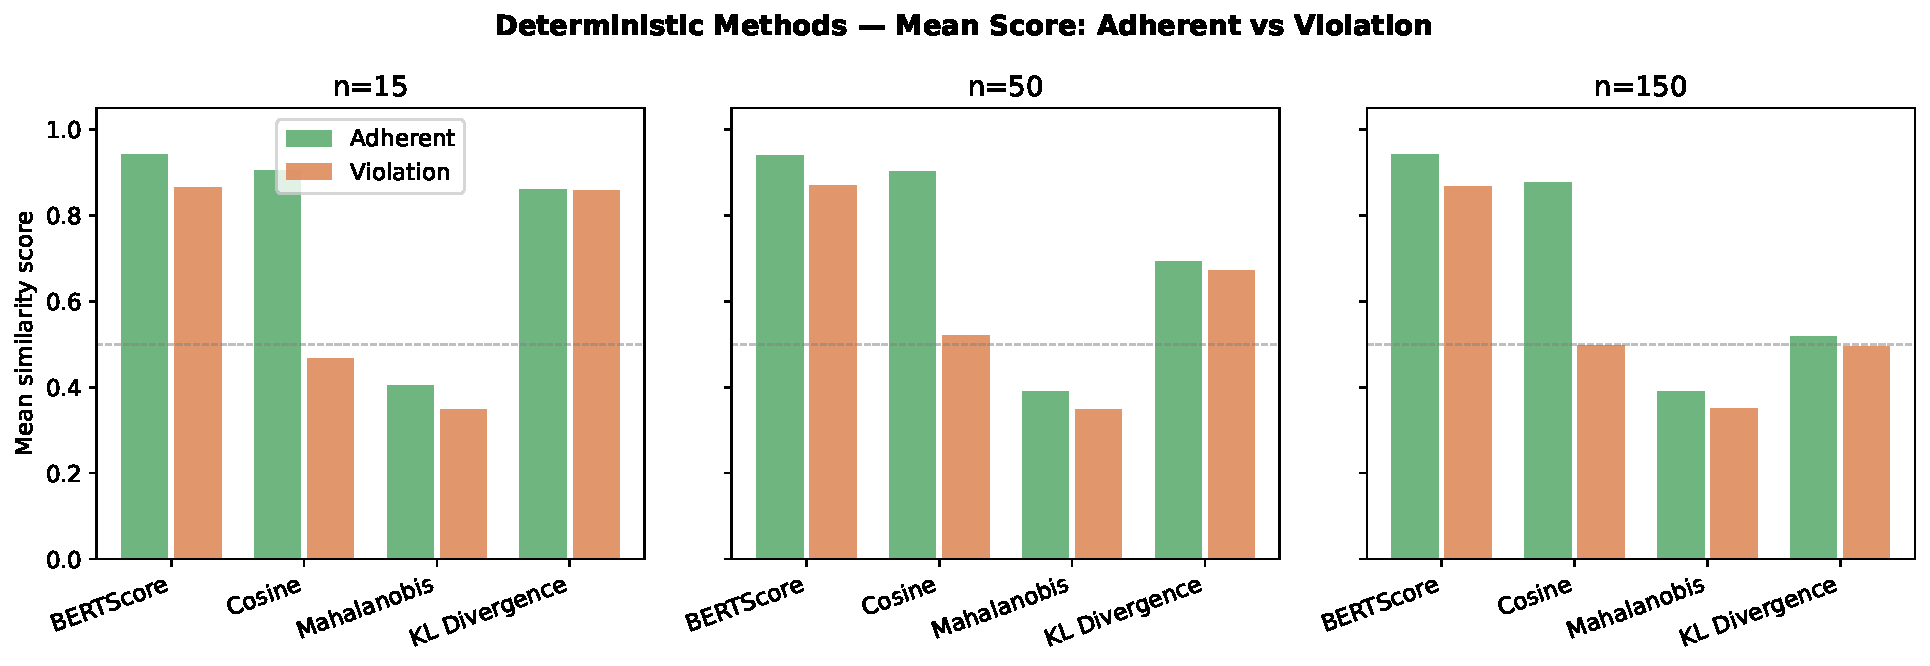
\includegraphics[width=\textwidth]{figures/fig1-similarity-by-label.pdf}
  \caption{Mean similarity score per class (adherent vs.\ violation) for
           BERTScore, Cosine similarity, Mahalanobis Distance, and KL Divergence
           across the three evaluation conditions.}
  \label{fig:similarity}
\end{figure}

Figure~\ref{fig:separation} shows the separation curve for Mahalanobis Distance,
KL Divergence, and PCA+Mahalanobis over intermediate sample sizes from $n = 15$
to $n = 150$. Mahalanobis separation declines monotonically from $+0.056$ to
$+0.041$. KL separation rises from near zero ($+0.002$) to $+0.023$.
PCA+Mahalanobis separation remains negative at every $n$, converging from
below towards zero without crossing it.

\begin{figure}[ht]
  \centering
  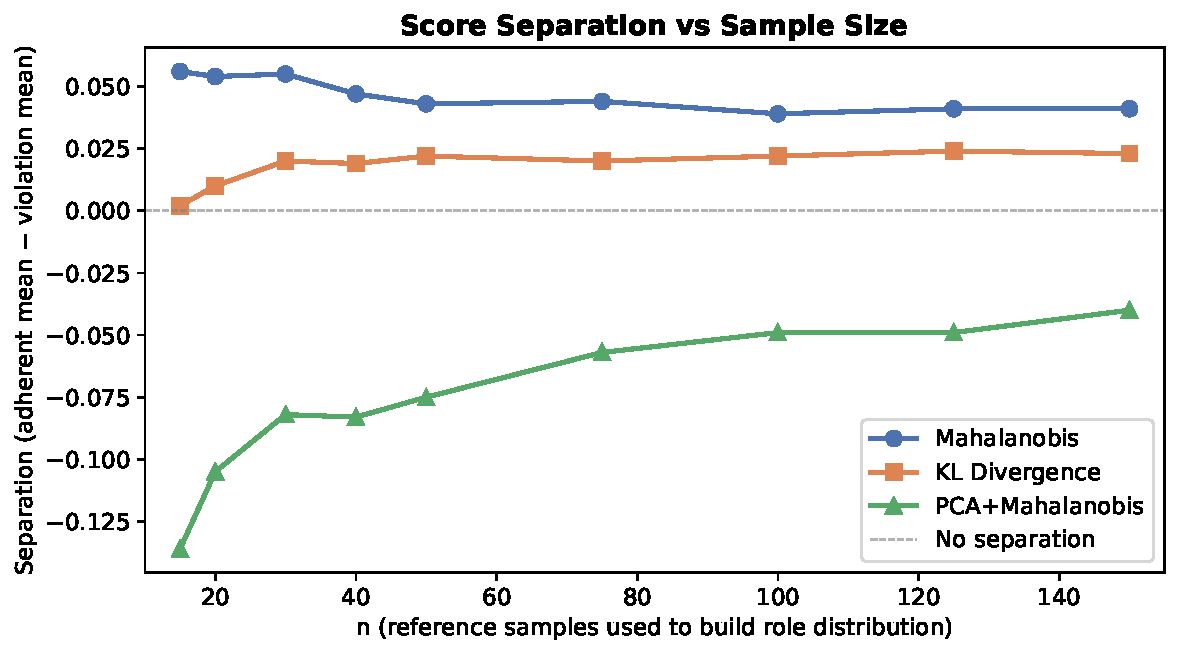
\includegraphics[width=0.82\textwidth]{figures/fig2-separation-curve.pdf}
  \caption{Score separation (adherent mean $-$ violation mean) as a function
           of sample size for Mahalanobis Distance, KL Divergence, and
           PCA+Mahalanobis. Positive values indicate the method ranks adherent
           responses higher on average; negative values indicate signal
           inversion.}
  \label{fig:separation}
\end{figure}

\subsection{Binary Classifiers}


\begin{table}[ht]
  \centering
  \caption{Binary classifiers: per-class F1, macro F1, and Cohen's $\kappa$.}
  \label{tab:bin_results}
  \begin{tabular}{llrrrr}
    \toprule
    \textbf{Method} & \textbf{Cond.} &
    \textbf{F1 adh.} & \textbf{F1 viol.} & \textbf{F1 macro} & \textbf{$\kappa$} \\
    \midrule
    NLI           & $n=15$  & 0.571 & 0.000 & 0.286 & 0.000 \\
                  & $n=50$  & 0.625 & 0.333 & 0.479 & 0.167 \\
                  & $n=150$ & 0.612 & 0.269 & 0.441 & 0.128 \\
    \addlinespace[3pt]
    LLM Judge     & $n=15$  & 1.000 & 1.000 & 1.000 & 1.000 \\
                  & $n=50$  & 0.974 & 0.984 & 0.979 & 0.958 \\
                  & $n=150$ & 0.974 & 0.984 & 0.979 & 0.958 \\
    \bottomrule
  \end{tabular}
\end{table}

\subsection{LLM Judge: Bootstrap Confidence Intervals}

The $n = 15$ result ($F_1 = 1.000$, $\kappa = 1.000$) reflects perfect
classification on a small and easy subsample and should not be taken as
the representative estimate. Table~\ref{tab:llm_ci} reports macro F1,
per-class F1, and Cohen's $\kappa$ with 95\% bootstrap confidence intervals
(1\,000 resamples, seed~42). The canonical result is $n = 150$:
$F_1^{\text{macro}} = 0.979$, $\kappa = 0.959$, CI\,[$0.952$,\,$1.000$].

\begin{table}[ht]
  \centering
  \caption{LLM Judge (\texttt{llama-3.3-70b-versatile}): macro F1, per-class F1,
           and Cohen's $\kappa$ with 95\% bootstrap confidence intervals
           (1\,000 resamples, seed~42).}
  \label{tab:llm_ci}
  \begin{tabular}{lrlrlrl}
    \toprule
    \textbf{Cond.} &
    \textbf{F1 macro} & \textbf{95\% CI} &
    \textbf{F1 adh.}  & \textbf{95\% CI} &
    \textbf{F1 viol.} & \textbf{95\% CI} \\
    \midrule
    $n=15$  & 1.000 & [1.000,\,1.000] & 1.000 & [1.000,\,1.000] & 1.000 & [1.000,\,1.000] \\
    $n=50$  & 0.979 & [0.934,\,1.000] & 0.975 & [0.914,\,1.000] & 0.984 & [0.947,\,1.000] \\
    $n=150$ & 0.979 & [0.952,\,1.000] & 0.975 & [0.942,\,1.000] & 0.984 & [0.963,\,1.000] \\
    \bottomrule
  \end{tabular}
\end{table}

\begin{figure}[ht]
  \centering
  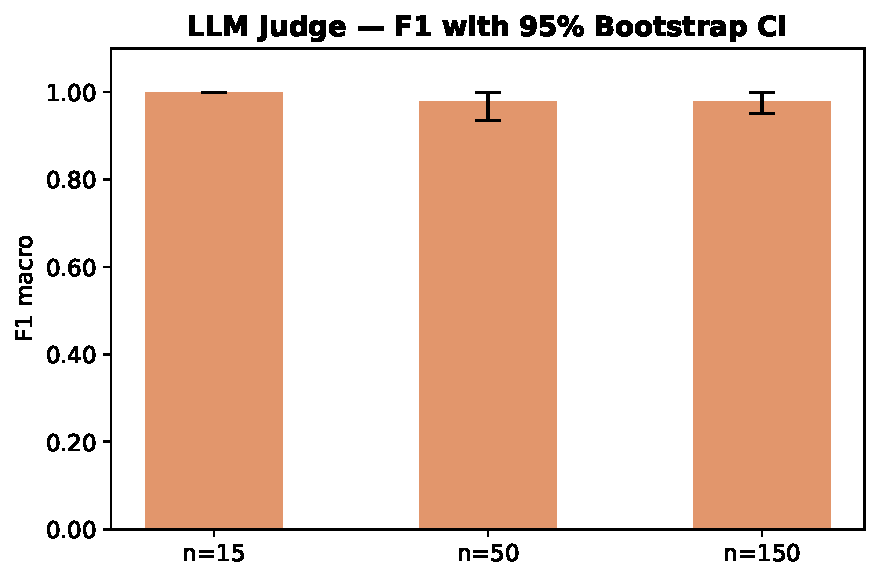
\includegraphics[width=0.6\textwidth]{figures/fig3-llm-judge-ci.pdf}
  \caption{LLM Judge macro F1 with 95\% bootstrap confidence intervals across
           evaluation conditions.}
  \label{fig:llm_ci}
\end{figure}
\newpage
% ---------------------------------------------------------------------------
\section{Discussion}
\label{sec:discussion}
% ---------------------------------------------------------------------------

\subsection{The Semantics Trap: Why AUC\,$\approx 1$ Is Not a Victory}

BERTScore, Cosine, and $k$-NN achieve AUC\,$\approx 1.0$ across all conditions.
Read naively, this looks like a definitive result. It is not. The benchmark
was constructed so that adherent responses are paraphrases of the ground truth
(semantically close by design) and violations are responses that mishandle or
ignore the request (semantically distinct by design). Any method that measures
semantic proximity to a per-turn ground-truth reference separates this benchmark
perfectly because separability was built into the construction, not discovered
by the method.

The per-class mean scores make the mechanism explicit: Cosine similarity
sits at $0.877$ for adherent responses and $0.497$ for violations at $n = 150$
--- the groups are nearly half a unit apart because adherent examples were
generated as paraphrases of the ground truth and violations were not. In
production, the hardest violations --- tone deviations and constructive
failures --- are precisely the ones where semantic similarity to the ground
truth is highest: a response may say the right things in the wrong register, or
omit the required resolution path while remaining topically on-role. Cosine
similarity would assign these a high score and miss the violation entirely.

The correct interpretation of deterministic methods with ground truth is that
they are \emph{semantic drift detectors}, not role adherence evaluators. They
are useful for monitoring whether response content deviates from an expected
reference, but they cannot substitute for a method that reads and understands
the role definition.

\subsection{Cosine vs.\ BERTScore: Practical Separation Matters}

Of the methods that reach AUC\,$\approx 1.0$, Cosine similarity achieves a
separation of $+0.380$ at $n = 150$ while BERTScore achieves only $+0.073$.
Although BERTScore operates at finer granularity (token-level contextual
embeddings versus sentence-level pooling), this additional resolution does not
translate to better group separation in this setup: the two groups are
sufficiently similar at the token level that BERTScore barely distinguishes
them in absolute terms, even though its ranking remains nearly perfect.

For a deployment requiring threshold-based binary classification, BERTScore's
small separation makes threshold selection fragile: a threshold at 0.90 and
one at 0.91 produce meaningfully different decisions. Cosine similarity, with
its large separation, is more robust to threshold choice.

$k$-NN is mathematically equivalent to Cosine in the single-reference-per-turn
setup used here ($k = 1$). Its advantage materialises when multiple valid
ground-truth responses exist per turn: the nearest-neighbour distance weights
the score towards the most similar acceptable response, gaining robustness that
a single-reference cosine comparison cannot provide.

\subsection{Mahalanobis Distance: Curse of Dimensionality Confirmed}

Mahalanobis Distance shows a monotonic degradation pattern: AUC is highest at
$n = 15$ ($0.963$) and declines to $0.856$ at $n = 150$. This is the opposite
of what standard statistical intuition would predict --- more data should
produce better distributional estimates, not worse ones.

The explanation is the concentration of measure in high-dimensional spaces
\citep{beyer1999nearest}. As $n$ grows, the estimated covariance of the
384-dimensional ground-truth embeddings converges towards the true distribution,
but in 384D all pairwise distances concentrate around a fixed value regardless
of class membership. The diagonal regularisation ($\lambda = 0.01$) partially
mitigates this at small $n$ by preventing covariance collapse; at larger $n$
the regularisation becomes relatively negligible and the concentration effect
dominates. This confirms the prediction embedded in H1: Mahalanobis Distance
is not viable for production deployments at standard embedding dimensions.

\subsection{PCA+Mahalanobis: A Structural Failure}

The PCA+Mahalanobis variant was motivated as a dimensionality reduction
solution to the concentration problem. The result is unambiguous: the method
inverts the adherence signal at every condition
(sep\,=\,$-0.136$ at $n = 15$, never crossing zero). AUC\,$= 0.000$ at
$n = 15$ means the method assigns higher scores to violations than to adherent
responses with perfect consistency.

The mechanism is structural. PCA decomposes the variance of the ground-truth
embedding matrix: the 32 retained principal components capture the directions
of maximum variance within the reference set. This transformation has no
relationship to the adherence-violation geometry --- it captures what varies
most \emph{among adherent examples}, not what separates adherent from violation.
In the compressed space, violation embeddings happen to project near the centroid
of the transformed reference distribution while adherent examples, spread across
the principal components, project further away.

More data partially corrects the PCA estimate (components become less dominated
by individual examples), which is why separation improves from $-0.136$ to
$-0.040$ as $n$ grows. But the structural distortion never reverses.
PCA+Mahalanobis is \textbf{not recommended} for any deployment scenario.
H2 is \textbf{refuted}: no deterministic method approaches the LLM Judge
at large $n$, and the methods that appear to do so via AUC are benefiting
from the benchmark artefact described above.

\subsection{KL Divergence: The Wrong Level of Abstraction}

KL Divergence operates on vocabulary distributions estimated from the
ground-truth corpus. Its near-random signal at $n = 15$ (AUC\,$= 0.537$)
is expected: with 15 turns the top-500 vocabulary distribution is too sparse
to be representative. As $n$ grows the distribution stabilises and AUC
converges to $0.877$ at $n = 150$.

The ceiling is not a sample-size problem --- it is a conceptual one. The role
violations in the benchmark (scope, tone, constructive failures) do not produce
distinctive vocabulary patterns. An agent that answers a question in the wrong
tone uses largely the same vocabulary as one that answers correctly. KL
Divergence is blind to this distinction because it operates at the lexical
level, not the semantic or pragmatic level. H4 cannot be confirmed from
aggregate binary classification; the convergence to AUC\,$= 0.877$ suggests
KL may serve as a rough vocabulary drift monitor but not as a primary adherence
detector.

\subsection{NLI: Insufficient for Role Adherence}

NLI achieves $F_1^{\text{macro}} = 0.441$ and $\kappa = 0.128$ at $n = 150$
--- better than chance but far below useful production thresholds. The model
correctly flags some explicit scope violations (responses that contradict
ground-truth assertions) but misses tone violations and constructive failures.
These failure types do not produce logical contradictions with the ground-truth
response: an agent that fails to offer a resolution path omits something, it
does not contradict anything. NLI's contradiction signal is a necessary but
insufficient condition for role violation. Performance is also unstable across
$n$: $\kappa$ drops from $0.167$ at $n = 50$ to $0.128$ at $n = 150$,
suggesting the threshold used for binary classification is not stable.

\subsection{LLM Judge: The Only Role-Aware Method}

The LLM Judge achieves $F_1^{\text{macro}} = 0.979$ at $n \geq 50$ with
bootstrap CI [$0.952$,\,$1.000$] at $n = 150$, $\kappa = 0.959$
[$0.904$,\,$1.000$]. It is the only evaluated method that reads the role
definition directly and evaluates the response against it. All other methods
operate on signals that are at best correlated with adherence; the judge
assesses adherence by definition and can detect tone violations and
constructive failures that are invisible to semantic similarity methods.

The practical costs are non-determinism (mitigated by fixing temperature to~0)
and per-call inference cost, both well-documented properties of LLM evaluation
\citep{zheng2023judging}.

\textbf{Judge model quality is a design variable.} The $F_1 = 0.979$ result
was obtained with \texttt{llama-3.3-70b-versatile}. A smaller model will
produce substantially different results. Reporting LLM Judge performance
without specifying the judge model is methodologically equivalent to reporting
a deterministic metric without specifying its embedding model: a necessary
parameter omitted. H3 cannot be directly tested with aggregate binary
classification; per-violation-type evaluation is identified as a direction for
future work.

% ---------------------------------------------------------------------------
\section{Configuration Parameters}
\label{sec:scoring_params}
% ---------------------------------------------------------------------------

The metric exposes the following parameters.

\textbf{\texttt{scoring\_method}} (default: \texttt{'llm\_judge'}) ---
selects the scoring function. \texttt{'llm\_judge'} (default) reads the
role definition directly and is the only option capable of detecting tone
violations and constructive failures. When ground-truth responses are
available, deterministic alternatives can be selected: \texttt{'cosine'}
and \texttt{'knn'} are recommended for cost-sensitive monitoring, with the
explicit caveat that they detect semantic drift from the reference rather
than role adherence per se; \texttt{'bertscore'} and \texttt{'nli'} are
also available. See Section~\ref{sec:results} for empirical characterisation
of each method.

\textbf{\texttt{output\_mode}} (default: \texttt{'binary'}) --- controls
the LLM judge output format. \texttt{'binary'} returns a hard $\{0, 1\}$
score per turn; \texttt{'continuous'} returns a float in $[0, 1]$. Binary
scoring is more consistent across calls. Continuous scoring is more
expressive but requires deliberate threshold selection. Applies only when
\texttt{scoring\_method='llm\_judge'}.

\textbf{\texttt{evaluation\_granularity}} (default: \texttt{'turn'}) ---
controls whether the judge evaluates each assistant turn with its prior
context (\texttt{'turn'}, one API call per turn, aligned with
Equation~\ref{eq:score}) or the full conversation in a single call
(\texttt{'conversation'}, lower cost, no per-turn breakdown). Applies only
when \texttt{scoring\_method='llm\_judge'}.

\textbf{\texttt{strict\_mode}} (default: \texttt{False}) --- when
\texttt{True}, the session passes only if every turn is adherent (session
score $= 1.0$). Intended for high-criticality deployments where partial
adherence is not acceptable.

\textbf{\texttt{threshold}} (default: 0.5) --- the minimum session score
required to mark the conversation as adherent. Ignored when
\texttt{strict\_mode=True}. In binary output mode a threshold of 0.5
requires that at least half of all turns are adherent; most relevant in
\texttt{output\_mode='continuous'}.

\textbf{\texttt{model}} --- the LLM used as judge. Follows the
\texttt{Guardian} abstraction in the Gaussia framework, allowing any
supported provider to be substituted. As shown in Section~\ref{sec:discussion},
judge model quality significantly affects detection performance and should
be treated as a first-class design parameter.

\textbf{\texttt{include\_reason}} (default: \texttt{False}) --- when
enabled, the judge returns a natural-language justification alongside each
per-turn score. Applies only when \texttt{scoring\_method='llm\_judge'}.

% ---------------------------------------------------------------------------
\section{Implementation Considerations}
% ---------------------------------------------------------------------------

The metric extends the \texttt{Gaussia} base class. The \texttt{batch()}
method iterates over each assistant turn in a session, dispatches to the
scoring function selected via \texttt{scoring\_method} (default:
\texttt{'llm\_judge'}), and appends a per-turn score. The session score is
the mean of per-turn scores (Equation~\ref{eq:score}).

The \texttt{chatbot\_role} field is read from the \texttt{Dataset} object
and passed as a string to all scoring methods and, when the judge path is
active, injected verbatim into the judge prompt.

Statistical mode compatibility (Frequentist and Bayesian) follows the existing
Gaussia pattern. No changes to the statistical layer are required.



% ---------------------------------------------------------------------------
\section{Future Work}
% ---------------------------------------------------------------------------

Two directions are identified for future development.

\textbf{Multimodal settings.} As conversational AI systems process images,
audio, and video alongside text, role adherence evaluation must generalise
beyond text-only responses. The LLM judge path extends naturally by
requiring a vision-capable model; the deterministic path would require
modality-appropriate similarity functions, such as CLIP-based similarity
\citep{radford2021clip} for image content.

\textbf{Re-evaluation on a larger and more diverse benchmark.} The current
benchmark is synthetic and scoped to a single domain. As discussed in
Section~\ref{sec:discussion}, the near-perfect AUC of semantic methods is
a structural property of this benchmark's construction rather than evidence
of genuine role understanding. A multi-domain benchmark with naturally
occurring violations --- including tone deviations that are semantically
close to adherent responses --- would provide a more demanding test for
all methods and may yield a different relative ordering.

% ---------------------------------------------------------------------------
\section{Conclusion}
% ---------------------------------------------------------------------------

We have proposed Role Adherence, a metric for the Gaussia evaluation framework
that measures how consistently an AI assistant maintains its assigned role
across a multi-turn conversation. The metric adopts a constructive definition of adherence, evaluates each
turn in full conversational context, and uses an LLM-as-a-judge as its
default scoring path. Deterministic semantic scoring is available as a
reproducible alternative when ground-truth reference responses are present.

Empirical evaluation on a controlled synthetic benchmark surfaces a distinction
with practical consequences: deterministic methods (BERTScore, Cosine, $k$-NN)
measure \emph{semantic proximity} to a reference response, not role adherence
per se. Their near-perfect AUC on the benchmark is a structural artefact of
how the benchmark was constructed, not evidence of role understanding. A
response that violates the role in tone or fails a constructive requirement
while remaining semantically close to the expected answer is invisible to
these methods. This finding motivates using deterministic methods only as
lightweight semantic drift monitors, not as primary adherence evaluators.

Among methods that model the reference distribution rather than individual
turn pairs, Mahalanobis Distance in high-dimensional embedding space degrades
monotonically with sample size (AUC $0.963 \to 0.856$), confirming the
curse of dimensionality. A PCA-based pre-reduction inverts the adherence signal
entirely and is not recommended. KL Divergence converges to a weak ceiling
(AUC $0.877$) because vocabulary overlap is a poor proxy for adherence.
The LLM Judge ($F_1 = 0.979$, $\kappa = 0.959$, CI [$0.952$,\,$1.000$]
at $n = 150$) is the only method that reliably detects all violation types,
at the cost of per-call inference and dependence on judge model quality ---
a variable that must be treated as a first-class design parameter.

Primary directions for future work are: (1)~per-violation-type evaluation to
test whether any deterministic method retains diagnostic value for specific
violation categories; (2)~multi-domain benchmarking beyond the single fintech
support agent domain used here; and (3)~cost-accuracy analysis of judge models
to characterise the tradeoff between inference cost and detection quality.

\bibliographystyle{plainnat}
\bibliography{refs}

\end{document}
